\section{Theorie}

Um den Leser den Einstieg in die Thematik zu erleichtern, wird zuerst einmal aufgezeigt, um was es sich bei einem Stubfilter genau handelt. Im Anschluss wird das typische Vorgehen einer Filterdimensionierung beschrieben, mit welchem ein Stubfilter realisiert werden kann.

\subsection{Stubfilter}

LC-Filter können in einem weiten Frequenzbereich eingesetzt werden. Jedoch wird bei konzentrierten Elementen zu höheren Frequenzen hin der Einfluss der parasitären Eigenschaften immer deutlicher, so dass hohe Anaforderungen an die Bauteilgüte gestellt werden müssen. Im GHZ-Bereich wird es daher zunehmend attraktiv, statt konzentrierten Kapazitäten und Induktivitäten verteilte Strukturen in Form von Leitungen zu verwenden. Man spricht dann von sogenannten Leitungsfilter.
%Quelle direktes Zitat: 
%https://books.google.ch/books?id=MTVQAgAAQBAJ&pg=PA203&lpg=PA203&dq=leitungsfilter+hochfrequenztechnik&source=bl&ots=Ljf0GRJkZt&sig=n-0G9H5VZ9iuPc2qepAATnjA47M&hl=de&sa=X&ved=0ahUKEwj38u-T79DUAhUSL1AKHUsyDNMQ6AEINTAB#v=onepage&q=leitungsfilter%20hochfrequenztechnik&f=false%

Es gibt verschiedene Arten um Leitungsfilter zu realisieren. Eine Möglichkeit der Realisierung ist das Stubfilter. Dieses Filter verwendet gleichlange kurzgeschlossenen Leitungen (TLSC) und leerlaufende Leitungen(TLOC), die nur an einem Ende verbunden werden. Das andere Ende wird entweder kurzgeschlossen oder eben offen gelassen. Bei diesen Leitungen handelt es sich um sogennante Stubs(Stichleitungen), die sich bei hohen Frequenzen wie reaktive Elemente (L,C) verhalten und somit die Realisierung eines Mikrowellenfilter ermöglichen.
%Der grosse Vorteil von Stubfiltern ist, das eine geschlossene Theorie zur Filtersynthese existiert. 

\newpage


\subsection{Ablauf Filterdimensionierung}

Der grundsätzliche Vorgehen bei der Filterdimensionierung ist bei fast allen Filtertypen gleich. Deshalb wird zuerst der allgemeinen Ablauf(Abb.\ref{fig:Ablauf_Filterdimensionierung_Allgemein}) der Filterdimensionierung beschrieben 

Der Entwurfsprozess jedes Filters beginnt mit der Filterspezifikation, welche mathematisch mit einer Funktion im Prototypbereich T(s) beschrieben wird. Aus dieser Funktion kann mit Hilfe einer Filtersynthese (rot) eine realisierbare Filterstruktur gefunden werden. Dabei ist zu beachten, dass  physikalische Randbedingungen einbezogen werden müssen, die nicht beliebig steile und beliebig verlustfreie Filtercharakteristiken erlauben.

Die Filtersynthesen unterschiedlicher Realisierungen haben gemeinsam, dass sie alle auf der klassischen LC-Filtersynthese basieren. Nach der LC-Filtersynthese liegt ein LC-Prototypfilter vor. Dieses LC-Prototypfilter wird bei der anschliessenden Filter-Realisierung mithilfe von unterschiedlichen Transformationen in den gewünschten Filter-Typ überführt(falls nötig). Für Elektroingenieure bekannte Transformationen sind z.B die billineare und die impulsinvariante Transformation, welche zur Überführung von einem LC-Filter in ein digitales Filter verwendet werden. Nach der Transformation ist die Filtersynthese abgeschlossen. Zuletzt wird das Filter aufgebaut wenn bei der Analyse alle Spezifikationen eingehalten wurden.

\begin{figure}[h!]
\centering
 	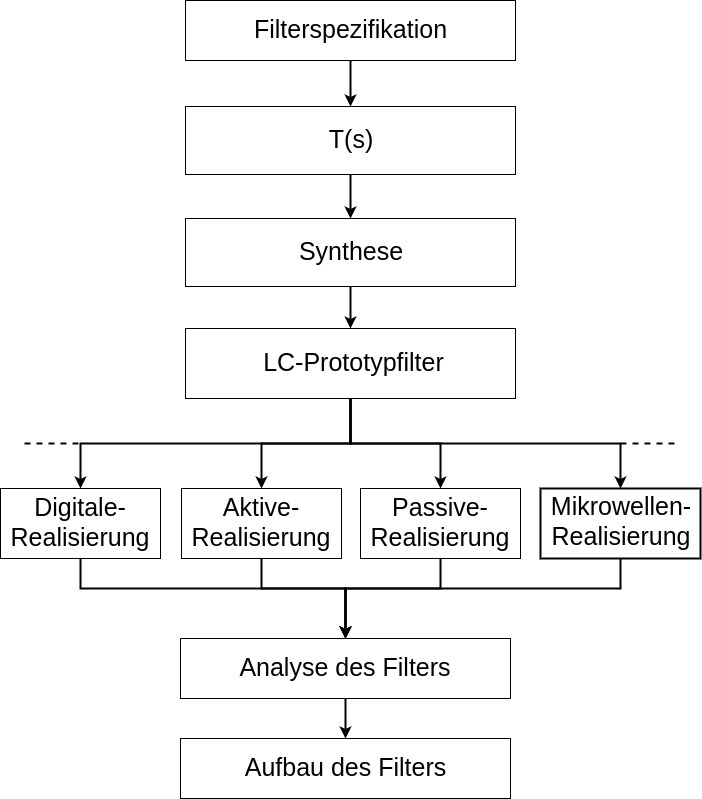
\includegraphics[width=0.5\textwidth]{Ablauf_Filterdimensionierung_Allgemein.png}
 	\caption{Ablauf Filterdimensionierung}
 	\label{fig:Ablauf_Filterdimensionierung_Allgemein}
\end{figure}

%Liegen keine speziellen Anforderungen an das Filter vor, so können Standardfilter(Butterworth, Chebyshev, Bessel und Cauer)verwendet werden. Die Reaktanzwerte, welche für die Beschreibung der Übertragungsfunktion des LC-Prototypfilters notwendig sind, sind aus Tabellen zu entnehmen. Werden Spezielle Anforderungen an das Filter gestellt, so eignen sich die Standardfilter nicht und es muss eine LC-Filtersynthese durchgeführt werden.

\paragraph{Realisierung Stubfilter}

Um schlussendlich vom LC-Prototypfilter zu einem realisierebaren Stubfilter zu gelangen sind zwei Transformationen notwendig: Die Richard's Transformation und die Kuroda Transformation.

Mit der Richard's Transformation können die konzentrierten Elemente (L,C) des Prototypfilter mit verteilte Elementen (Stubs) ersetzt werden. Nach dieser Transformation spricht man von einem Stubfilter. Das Problem ist aber, dass sich dieses Filter nicht realisieren lässt, weil sich alle Stubs am gleichen Ort befinden. 

Deshalb wird im Anschluss die Kuroda Transformation verwendet,  um eine physikalische Distanz zwischen
den  Stubs  zu  schaffen, damit das Filter auch in Realit\"at umgesetzt  werden  kann.





















